\documentclass[11pt, a4paper]{article}\usepackage[]{graphicx}\usepackage[]{xcolor}
% maxwidth is the original width if it is less than linewidth
% otherwise use linewidth (to make sure the graphics do not exceed the margin)
\makeatletter
\def\maxwidth{ %
  \ifdim\Gin@nat@width>\linewidth
    \linewidth
  \else
    \Gin@nat@width
  \fi
}
\makeatother

\definecolor{fgcolor}{rgb}{0.345, 0.345, 0.345}
\newcommand{\hlnum}[1]{\textcolor[rgb]{0.686,0.059,0.569}{#1}}%
\newcommand{\hlsng}[1]{\textcolor[rgb]{0.192,0.494,0.8}{#1}}%
\newcommand{\hlcom}[1]{\textcolor[rgb]{0.678,0.584,0.686}{\textit{#1}}}%
\newcommand{\hlopt}[1]{\textcolor[rgb]{0,0,0}{#1}}%
\newcommand{\hldef}[1]{\textcolor[rgb]{0.345,0.345,0.345}{#1}}%
\newcommand{\hlkwa}[1]{\textcolor[rgb]{0.161,0.373,0.58}{\textbf{#1}}}%
\newcommand{\hlkwb}[1]{\textcolor[rgb]{0.69,0.353,0.396}{#1}}%
\newcommand{\hlkwc}[1]{\textcolor[rgb]{0.333,0.667,0.333}{#1}}%
\newcommand{\hlkwd}[1]{\textcolor[rgb]{0.737,0.353,0.396}{\textbf{#1}}}%
\let\hlipl\hlkwb

\usepackage{framed}
\makeatletter
\newenvironment{kframe}{%
 \def\at@end@of@kframe{}%
 \ifinner\ifhmode%
  \def\at@end@of@kframe{\end{minipage}}%
  \begin{minipage}{\columnwidth}%
 \fi\fi%
 \def\FrameCommand##1{\hskip\@totalleftmargin \hskip-\fboxsep
 \colorbox{shadecolor}{##1}\hskip-\fboxsep
     % There is no \\@totalrightmargin, so:
     \hskip-\linewidth \hskip-\@totalleftmargin \hskip\columnwidth}%
 \MakeFramed {\advance\hsize-\width
   \@totalleftmargin\z@ \linewidth\hsize
   \@setminipage}}%
 {\par\unskip\endMakeFramed%
 \at@end@of@kframe}
\makeatother

\definecolor{shadecolor}{rgb}{.97, .97, .97}
\definecolor{messagecolor}{rgb}{0, 0, 0}
\definecolor{warningcolor}{rgb}{1, 0, 1}
\definecolor{errorcolor}{rgb}{1, 0, 0}
\newenvironment{knitrout}{}{} % an empty environment to be redefined in TeX

\usepackage{alltt}

\usepackage[top = 1 in, bottom = 1 in, left = 0.75 in, right = 0.75 in]{geometry}

\usepackage{amsmath, amssymb, amsfonts}
\usepackage{enumerate}
\usepackage{array}
\usepackage{multirow}
\usepackage{dingbat}
\usepackage{fontawesome5}
\usepackage{tasks}
\usepackage{bbding}
\usepackage{twemojis}
% how to use bull's eye ----- \scalebox{2.0}{\twemoji{bullseye}}
\usepackage{fontspec}
\usepackage{customdice}
% how to put dice face ------ \dice{2}

\title{MSMS 105 : Practical}
\author{Ananda Biswas}
\date{25 November, 2024}

\newfontface\ifr{IndieFlower-Regular.ttf}
% how to use ---- {\ifr write text here}
\IfFileExists{upquote.sty}{\usepackage{upquote}}{}
\begin{document}

\maketitle


\section*{\faArrowAltCircleRight[regular] \textcolor{blue}{Question}}

\hspace{1cm} A class of 15 students has their test scores recorded in four subjects - Math, Science, English and History. Analyze the pairwise Pearson Correlation coefficients between these subjects to determine the relationships between them. Present the data and results of the analysis.

\begin{table}[!htbp]
\def\arraystretch{1.5}

\begin{center}
\begin{tabular}{|c||c|c|c|c|c|c|c|c|c|c|c|c|c|c|c|}

\hline

Student & 1 & 2 & 3 & 4 & 5 & 6 & 7 & 8 & 9 & 10 & 11 & 12 & 13 & 14 & 15 \\

\hline
\hline

Math & 67 & 88 & 77 & 92 & 81 & 76 & 89 & 72 & 95 & 68 & 74 & 85 & 80 & 90 & 79 \\

\hline

Science & 93 & 63 & 96 & 85 & 72 & 88 & 78 & 91 & 84 & 75 & 89 & 80 & 87 & 94 & 76 \\

\hline

English & 83 & 87 & 85 & 92 & 76 & 88 & 82 & 74 & 86 & 81 & 79 & 84 & 90 & 77 & 80 \\

\hline

History & 87 & 85 & 75 & 80 & 79 & 86 & 83 & 82 & 91 & 88 & 77 & 90 & 78 & 84 & 89 \\

\hline

\end{tabular}
\end{center}
\end{table}




\section*{\faArrowAltCircleRight[regular] \textcolor{blue}{R Program, Plot and Interpretation}}

\begin{knitrout}\footnotesize
\definecolor{shadecolor}{rgb}{0.969, 0.969, 0.969}\color{fgcolor}\begin{kframe}
\begin{alltt}
\hldef{df} \hlkwb{<-} \hlkwd{read.csv}\hldef{(}\hlsng{'https://raw.githubusercontent.com/sakunisgithub/data_sets/refs/heads/master/test_scores.csv'}\hldef{)}
\end{alltt}
\end{kframe}
\end{knitrout}

\begin{knitrout}
\definecolor{shadecolor}{rgb}{0.969, 0.969, 0.969}\color{fgcolor}\begin{kframe}
\begin{alltt}
\hldef{my_mean} \hlkwb{<-} \hlkwa{function}\hldef{(}\hlkwc{vec}\hldef{)\{}
  \hldef{s} \hlkwb{<-} \hlnum{0}
  \hlkwa{for} \hldef{(i} \hlkwa{in} \hlnum{1}\hlopt{:}\hlkwd{length}\hldef{(vec)) \{}
    \hldef{s} \hlkwb{<-} \hldef{s} \hlopt{+} \hldef{vec[i]}
  \hldef{\}}
  \hlkwd{return}\hldef{(s}\hlopt{/}\hlkwd{length}\hldef{(vec))}
\hldef{\}}
\end{alltt}
\end{kframe}
\end{knitrout}

\begin{knitrout}
\definecolor{shadecolor}{rgb}{0.969, 0.969, 0.969}\color{fgcolor}\begin{kframe}
\begin{alltt}
\hldef{my_cov} \hlkwb{<-} \hlkwa{function}\hldef{(}\hlkwc{vec1}\hldef{,} \hlkwc{vec2}\hldef{)\{}
  \hldef{s} \hlkwb{<-} \hlnum{0}
  \hlkwa{for} \hldef{(i} \hlkwa{in} \hlnum{1}\hlopt{:}\hlkwd{length}\hldef{(vec1)) \{}
    \hldef{s} \hlkwb{<-} \hldef{s} \hlopt{+} \hldef{(vec1[i]} \hlopt{-} \hlkwd{my_mean}\hldef{(vec1))} \hlopt{*} \hldef{(vec2[i]} \hlopt{-} \hlkwd{my_mean}\hldef{(vec2))}
  \hldef{\}}
  \hlkwd{return}\hldef{(s}\hlopt{/}\hlkwd{length}\hldef{(vec1))}
\hldef{\}}
\end{alltt}
\end{kframe}
\end{knitrout}

\begin{knitrout}
\definecolor{shadecolor}{rgb}{0.969, 0.969, 0.969}\color{fgcolor}\begin{kframe}
\begin{alltt}
\hldef{my_var} \hlkwb{<-} \hlkwa{function}\hldef{(}\hlkwc{vec}\hldef{)\{}
  \hldef{s} \hlkwb{<-} \hlnum{0}
  \hlkwa{for} \hldef{(i} \hlkwa{in} \hlnum{1}\hlopt{:}\hlkwd{length}\hldef{(vec)) \{}
    \hldef{s} \hlkwb{<-} \hldef{s} \hlopt{+} \hldef{(vec[i]} \hlopt{-} \hlkwd{my_mean}\hldef{(vec))}\hlopt{^}\hlnum{2}
  \hldef{\}}
  \hlkwd{return}\hldef{(s}\hlopt{/}\hlkwd{length}\hldef{(vec))}
\hldef{\}}
\end{alltt}
\end{kframe}
\end{knitrout}


\begin{knitrout}
\definecolor{shadecolor}{rgb}{0.969, 0.969, 0.969}\color{fgcolor}\begin{kframe}
\begin{alltt}
\hldef{my_corr} \hlkwb{<-} \hlkwa{function}\hldef{(}\hlkwc{vec1}\hldef{,} \hlkwc{vec2}\hldef{)\{}
  \hldef{temp} \hlkwb{<-} \hlkwd{my_cov}\hldef{(vec1, vec2)} \hlopt{/} \hlkwd{sqrt}\hldef{(}\hlkwd{my_var}\hldef{(vec1)} \hlopt{*} \hlkwd{my_var}\hldef{(vec2))}
  \hlkwd{return}\hldef{(temp)}
\hldef{\}}
\end{alltt}
\end{kframe}
\end{knitrout}

\begin{knitrout}
\definecolor{shadecolor}{rgb}{0.969, 0.969, 0.969}\color{fgcolor}\begin{kframe}
\begin{alltt}
\hlkwa{for} \hldef{(i} \hlkwa{in} \hlnum{1}\hlopt{:}\hlnum{4}\hldef{) \{}
  \hldef{temp} \hlkwb{<-} \hlkwd{paste}\hldef{(}\hlsng{"Average score in"}\hldef{,} \hlkwd{names}\hldef{(df)[i}\hlopt{+}\hlnum{1}\hldef{],} \hlsng{"is"}\hldef{,} \hlkwd{my_mean}\hldef{(df[,i}\hlopt{+}\hlnum{1}\hldef{]),} \hlkwc{sep} \hldef{=} \hlsng{" "}\hldef{)}
  \hlkwd{print}\hldef{(temp)}
\hldef{\}}
\end{alltt}
\begin{verbatim}
## [1] "Average score in Mathematics is 80.9333333333333"
## [1] "Average score in Science is 83.4"
## [1] "Average score in English is 82.9333333333333"
## [1] "Average score in History is 83.6"
\end{verbatim}
\end{kframe}
\end{knitrout}

\begin{knitrout}
\definecolor{shadecolor}{rgb}{0.969, 0.969, 0.969}\color{fgcolor}\begin{kframe}
\begin{alltt}
\hlkwa{for} \hldef{(i} \hlkwa{in} \hlnum{2}\hlopt{:}\hlnum{4}\hldef{) \{}
  \hlkwa{for} \hldef{(j} \hlkwa{in} \hldef{(i}\hlopt{+}\hlnum{1}\hldef{)}\hlopt{:}\hlnum{5}\hldef{) \{}
    \hldef{temp} \hlkwb{<-} \hlkwd{paste}\hldef{(}\hlsng{"Correlation between"}\hldef{,} \hlkwd{names}\hldef{(df)[i],} \hlsng{"and"}\hldef{,} \hlkwd{names}\hldef{(df)[j],} \hlsng{"is"}\hldef{,}
                  \hlkwd{my_corr}\hldef{(df[,i], df[,j]),} \hlkwc{sep} \hldef{=} \hlsng{" "}\hldef{)}
    \hlkwd{print}\hldef{(temp)}
  \hldef{\}}
\hldef{\}}
\end{alltt}
\begin{verbatim}
## [1] "Correlation between Mathematics and Science is -0.251550054947875"
## [1] "Correlation between Mathematics and English is 0.333064725095778"
## [1] "Correlation between Mathematics and History is 0.125201003384908"
## [1] "Correlation between Science and English is -0.0378386398631776"
## [1] "Correlation between Science and History is -0.312589056194899"
## [1] "Correlation between English and History is 0.00986489121169494"
\end{verbatim}
\end{kframe}
\end{knitrout}

\begin{knitrout}
\definecolor{shadecolor}{rgb}{0.969, 0.969, 0.969}\color{fgcolor}\begin{kframe}
\begin{alltt}
\hlkwd{library}\hldef{(tidyverse)}
\end{alltt}
\end{kframe}
\end{knitrout}

\begin{knitrout}
\definecolor{shadecolor}{rgb}{0.969, 0.969, 0.969}\color{fgcolor}\begin{kframe}
\begin{alltt}
\hlkwd{library}\hldef{(ggcorrplot)}

\hldef{cor_df} \hlkwb{<-} \hlkwd{cor}\hldef{(df[,}\hlnum{2}\hlopt{:}\hlnum{5}\hldef{])}

\hlkwd{ggcorrplot}\hldef{(cor_df,}
           \hlkwc{method} \hldef{=} \hlsng{"square"}\hldef{,}
           \hlkwc{type} \hldef{=} \hlsng{"lower"}\hldef{,}
           \hlkwc{lab} \hldef{=} \hlnum{TRUE}\hldef{,}
           \hlkwc{lab_col} \hldef{=} \hlsng{"black"}\hldef{,}
           \hlkwc{lab_size} \hldef{=} \hlnum{5}\hldef{,}
           \hlkwc{outline.color} \hldef{=} \hlsng{"white"}\hldef{,}
           \hlkwc{tl.cex} \hldef{=} \hlnum{20}\hldef{,}
           \hlkwc{legend.title} \hldef{=} \hlsng{""}\hldef{)} \hlopt{+}
  \hlkwd{theme}\hldef{(}\hlkwc{axis.text.x} \hldef{=} \hlkwd{element_text}\hldef{(}\hlkwc{angle} \hldef{=} \hlnum{90}\hldef{,} \hlkwc{hjust} \hldef{=} \hlnum{1}\hldef{),}
        \hlkwc{panel.background} \hldef{=} \hlkwd{element_rect}\hldef{(}\hlkwc{fill} \hldef{=} \hlsng{"white"}\hldef{),}
        \hlkwc{panel.grid.major} \hldef{=} \hlkwd{element_blank}\hldef{(),}
        \hlkwc{panel.border} \hldef{=} \hlkwd{element_blank}\hldef{(),}
        \hlkwc{legend.key.height} \hldef{=} \hlkwd{unit}\hldef{(}\hlnum{3}\hldef{,} \hlsng{'cm'}\hldef{),}
        \hlkwc{legend.key.width} \hldef{=} \hlkwd{unit}\hldef{(}\hlnum{1}\hldef{,} \hlsng{'cm'}\hldef{))}
\end{alltt}
\end{kframe}
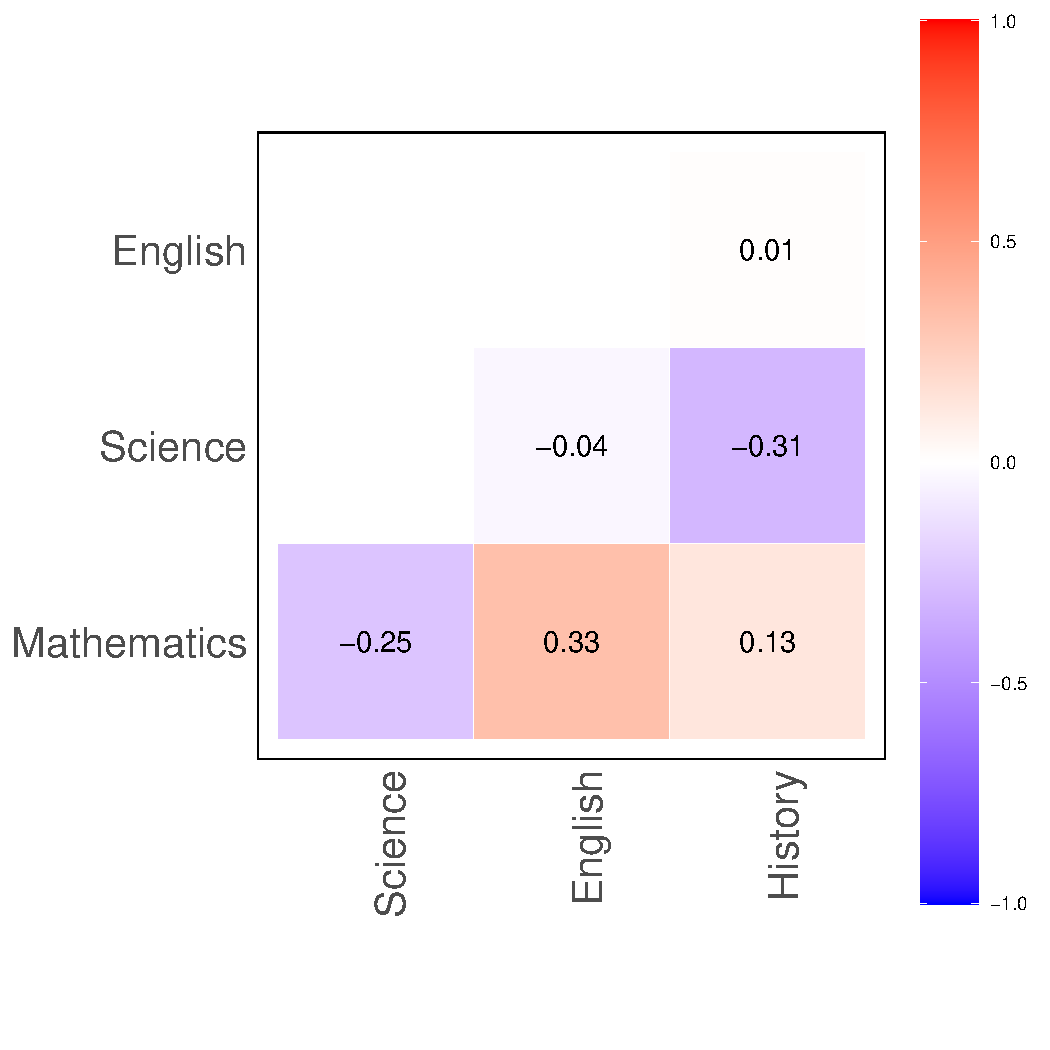
\includegraphics[width=\maxwidth]{figure/unnamed-chunk-9-1} 
\end{knitrout}

\begin{knitrout}
\definecolor{shadecolor}{rgb}{0.969, 0.969, 0.969}\color{fgcolor}\begin{kframe}
\begin{alltt}
\hlkwd{library}\hldef{(GGally)}
\end{alltt}
\end{kframe}
\end{knitrout}

\begin{knitrout}
\definecolor{shadecolor}{rgb}{0.969, 0.969, 0.969}\color{fgcolor}\begin{kframe}
\begin{alltt}
\hlkwd{ggpairs}\hldef{(df,}
        \hlkwc{columns} \hldef{=} \hlnum{2}\hlopt{:}\hlnum{5}\hldef{,}
        \hlkwc{upper} \hldef{=} \hlkwd{list}\hldef{(}\hlkwc{continuous} \hldef{=} \hlsng{"points"}\hldef{),} \hlkwc{legend} \hldef{=} \hlkwd{c}\hldef{(}\hlnum{1}\hldef{,}\hlnum{1}\hldef{))} \hlopt{+}
  \hlkwd{scale_alpha}\hldef{(}\hlkwc{guide} \hldef{=} \hlsng{"none"}\hldef{)} \hlopt{+}
  \hlkwd{theme}\hldef{(}\hlkwc{axis.text.x} \hldef{=} \hlkwd{element_text}\hldef{(}\hlkwc{angle} \hldef{=} \hlnum{45}\hldef{,} \hlkwc{hjust} \hldef{=} \hlnum{1}\hldef{))}
\end{alltt}
\end{kframe}
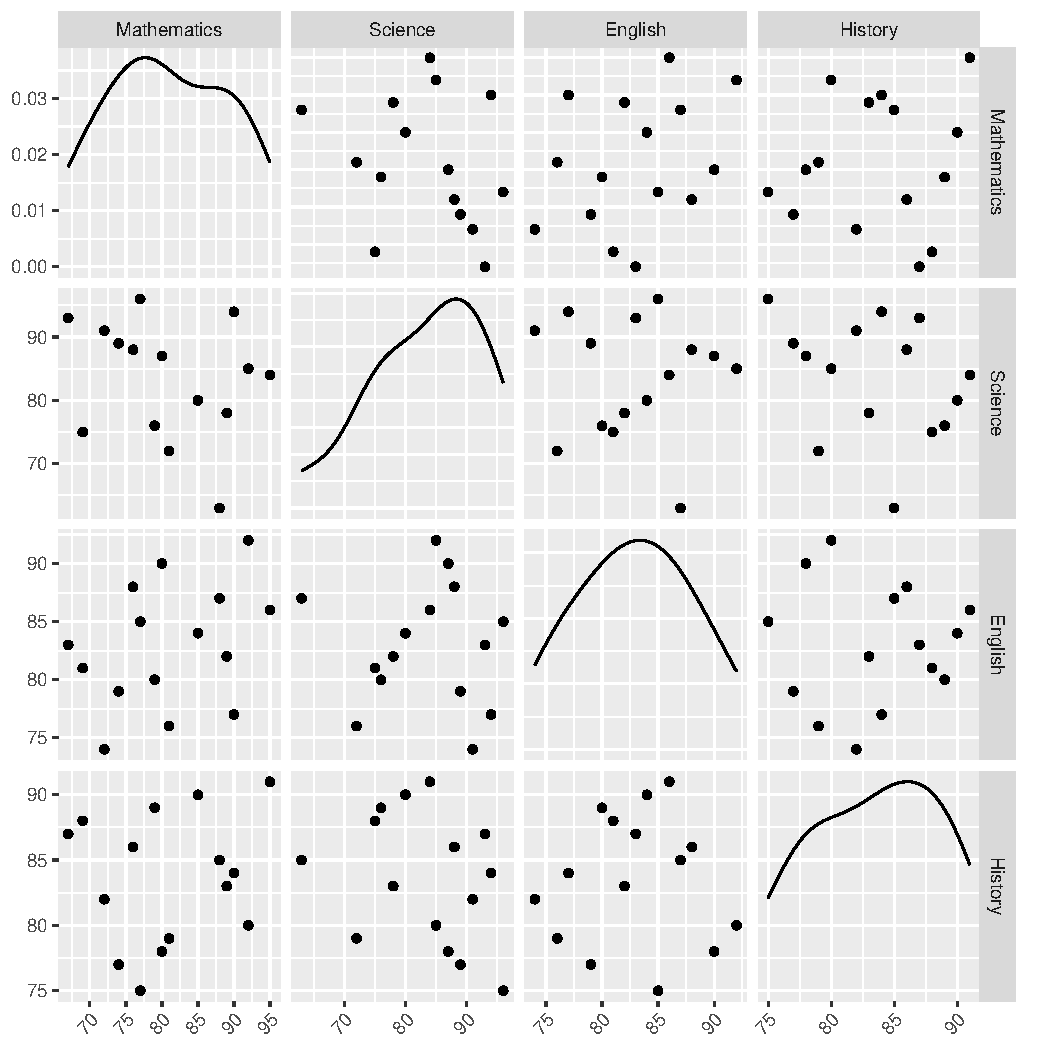
\includegraphics[width=\maxwidth]{figure/unnamed-chunk-11-1} 
\end{knitrout}



\section*{\faArrowAltCircleRight[regular] \textcolor{blue}{Conclusion}}

\smallpencil \hspace{0.1cm} {\ifr No significant linear or curvi-linear pattern is found in the scatterplots of the scores of different subjects.}

\end{document}
